%introduction

Software testing is a crucial part of systems that run our lives. Industries that rely on predicting consumer habit trends or dispatching taxi cars are deeply affected when their software fails to provide accurate results. The gravity of this trust is even greater in safety-critical programs controlling gas-leak shut off valves or anesthetic delivery machines. Consequently, before these pieces of software are deployed, they must be checked and tested as rigorously as necessary, but no more. The breadth and completeness of testing is directly proportional to how much damage could occur if the software malfunctioned. The software must eventually reach production (used in the hands of the customer or used in industrial practice ``for real'') and cannot spend too much of its lifetime under test. Therefore, cost and convenience of testing is an important consideration in determining the rigor of testing. Neither cost nor convenience is really ever that low because few tools exist to make that job easier, so software testing remains largely overlooked in industrial practice; developing new techniques is too expensive and time-consuming and that is why engineers don't do it. 

A key component of getting correct results is knowledge of what that correctness looks like. Developers and testers must be careful not to confuse code that compiles and runs without errors with code that garners accurate results. To find accurate results, testers need an oracle, which is a way of determining how close the actual result of a program is to the expected result. Figure \ref{fig:workflow} illustrates the divergence. Unsurprisingly, attaining and checking this oracle is difficult. Given a particular input to a program, a tester must know what the expected result even is. 
\begin{wrapfigure}{l}{0.65\textwidth}
\centering
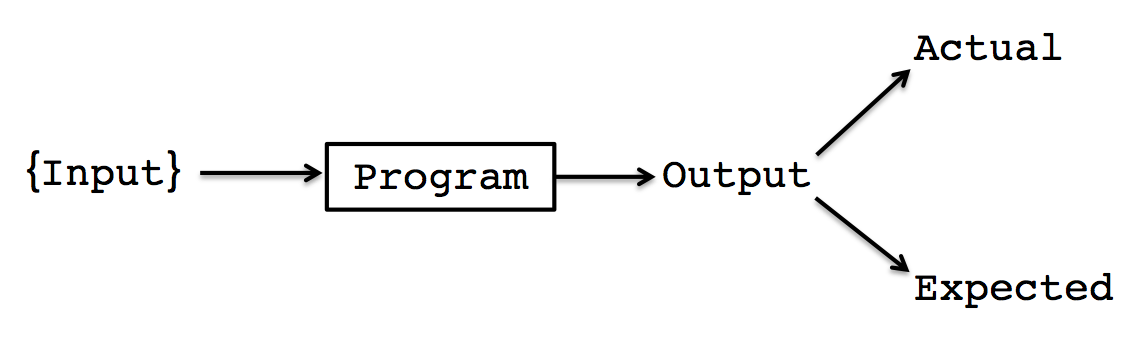
\includegraphics[width=90mm,scale=0.5]{diagram.png}
\caption{Basic Workflow of a software program}
\label{fig:workflow}
\end{wrapfigure}
Then, she must know how to read or understand the actual result and be able to compare it to the expected. Consequently, many companies often build the role of tester into the role of developer, since the developer has the most intimate knowledge of the design and implementation of the software, and therefore has a better sense of what the output of the program garners. Even then, it may be impossible to describe the ideal expected output of the program.

However, there are some basic oracles and trends that can be tested that can offer high confidence that the program functions as anticipated. For example, it might be difficult to know what a piece of software should do, but significantly easier to know what the software should not do. Online banking software should not deposit millions of dollars into the account of a blacklisted felon.
Another major challenge in software testing is the need to know all the possible situations you may want to test for. In the automobile simulation, a tester does not want to just test for braking and accelerating, they might want to test turn-signaling and beeping and brake-lighting, and also combinations of those tests to make sure that the beeping sensor does not accidentally disable the brake pedal capability. Knowing and describing every single situation may be unknown to the tester; they may not even think that that is a situation they have to test for. What is known as the ``happy path'', the operational choice that most represents the typical testing scenario, is certainly necessary for testing the program’s reliability, but it does not find the bugs. Outlier situations find the bugs. Identifying all these possible outlier situations is \textbf{Problem One}.

The next problem is writing the actual test data itself. A symbolic description of the test must be turned into an actual concrete input to the software. A test vector checking that beeping does not disable braking must be turned into ``beeping=5s\&\&braking=true'' or whatever discrete format the SUT requires. This is not a step that should be done manually. For example, VisIt, a graphical visualization tool~\cite{VisIt}, is capable of handling several gigabyte files, and no tester wants to or even could write three gigabytes of data points by hand just to test something. This is \textbf{Problem Two}.

It is significantly easier to describe the trend of a certain test than it is to create the hundreds (if not more) data points that fit that description. Therefore, the goal of this paper is to bridge that gap. It aims to aid the tester in designing and creating test suites so as to provide automation in the testing process. The reality of the software development environment means that solutions must be adopted to ensure accurate software while still maintaining a practical timeline and budget. 

Finally, it is important to consider the necessity of generating this data in the first place. Gotterbarn remarks, ``Insufficient data is not a problem''~\cite{Gotterbarn:2016:CFC:2874239.2874248}, implying that data exists for most programs we want to test. For example, consider an ocean temperature monitoring software that has predictive power in future local hot spots or cold zones. Ocean temperature data points do exist, and the missing points can likely be interpolated quite easily. But this is a sample size of one. To be sure the temperature projection software is robust, the tester would want to study a variety of circumstances and possibilities – situations that do not even exist. They might perhaps want to study temperature diffusion trends as a result of a significant event 30 years from now. Data for that particular test case has to be created.